\begin{MyArticle}[enhanced, tikz={rotate=0}]{Top Quark, Last Piece of Matter, Appears to Be in Place}
  \begin{multicols}{2}
    We establish the existence of the top quark using a 67 pb$^{-1}$ data
    sample of pp collisions at $\sqrt{s} = 1.8$ TeV collected with the Collider
    Detector at Fermilab (CDF). Employing techniques similar to those we
    previously published, we observe a signal consistent with $t\bar{t}$ decay to
    $WWbb$, but inconsistent with the background prediction by
    4.8$\sigma$. Additional evidence for the top quark is provided by a peak in
    the reconstructed mass distribution. We measure the top quark mass
    to be $176 \pm 8 (\text{stat.}) \pm 10 (\text{sys.})$ GeV/c$^{2}$,
    and the $t\bar{t}$ production cross section to be
    $6.8^{+3.6}_{-2.4}$ pb.
    % ========================
    \begin{figure}
      \begin{center}
        \vspace{-0.2in}
        \leavevmode
        %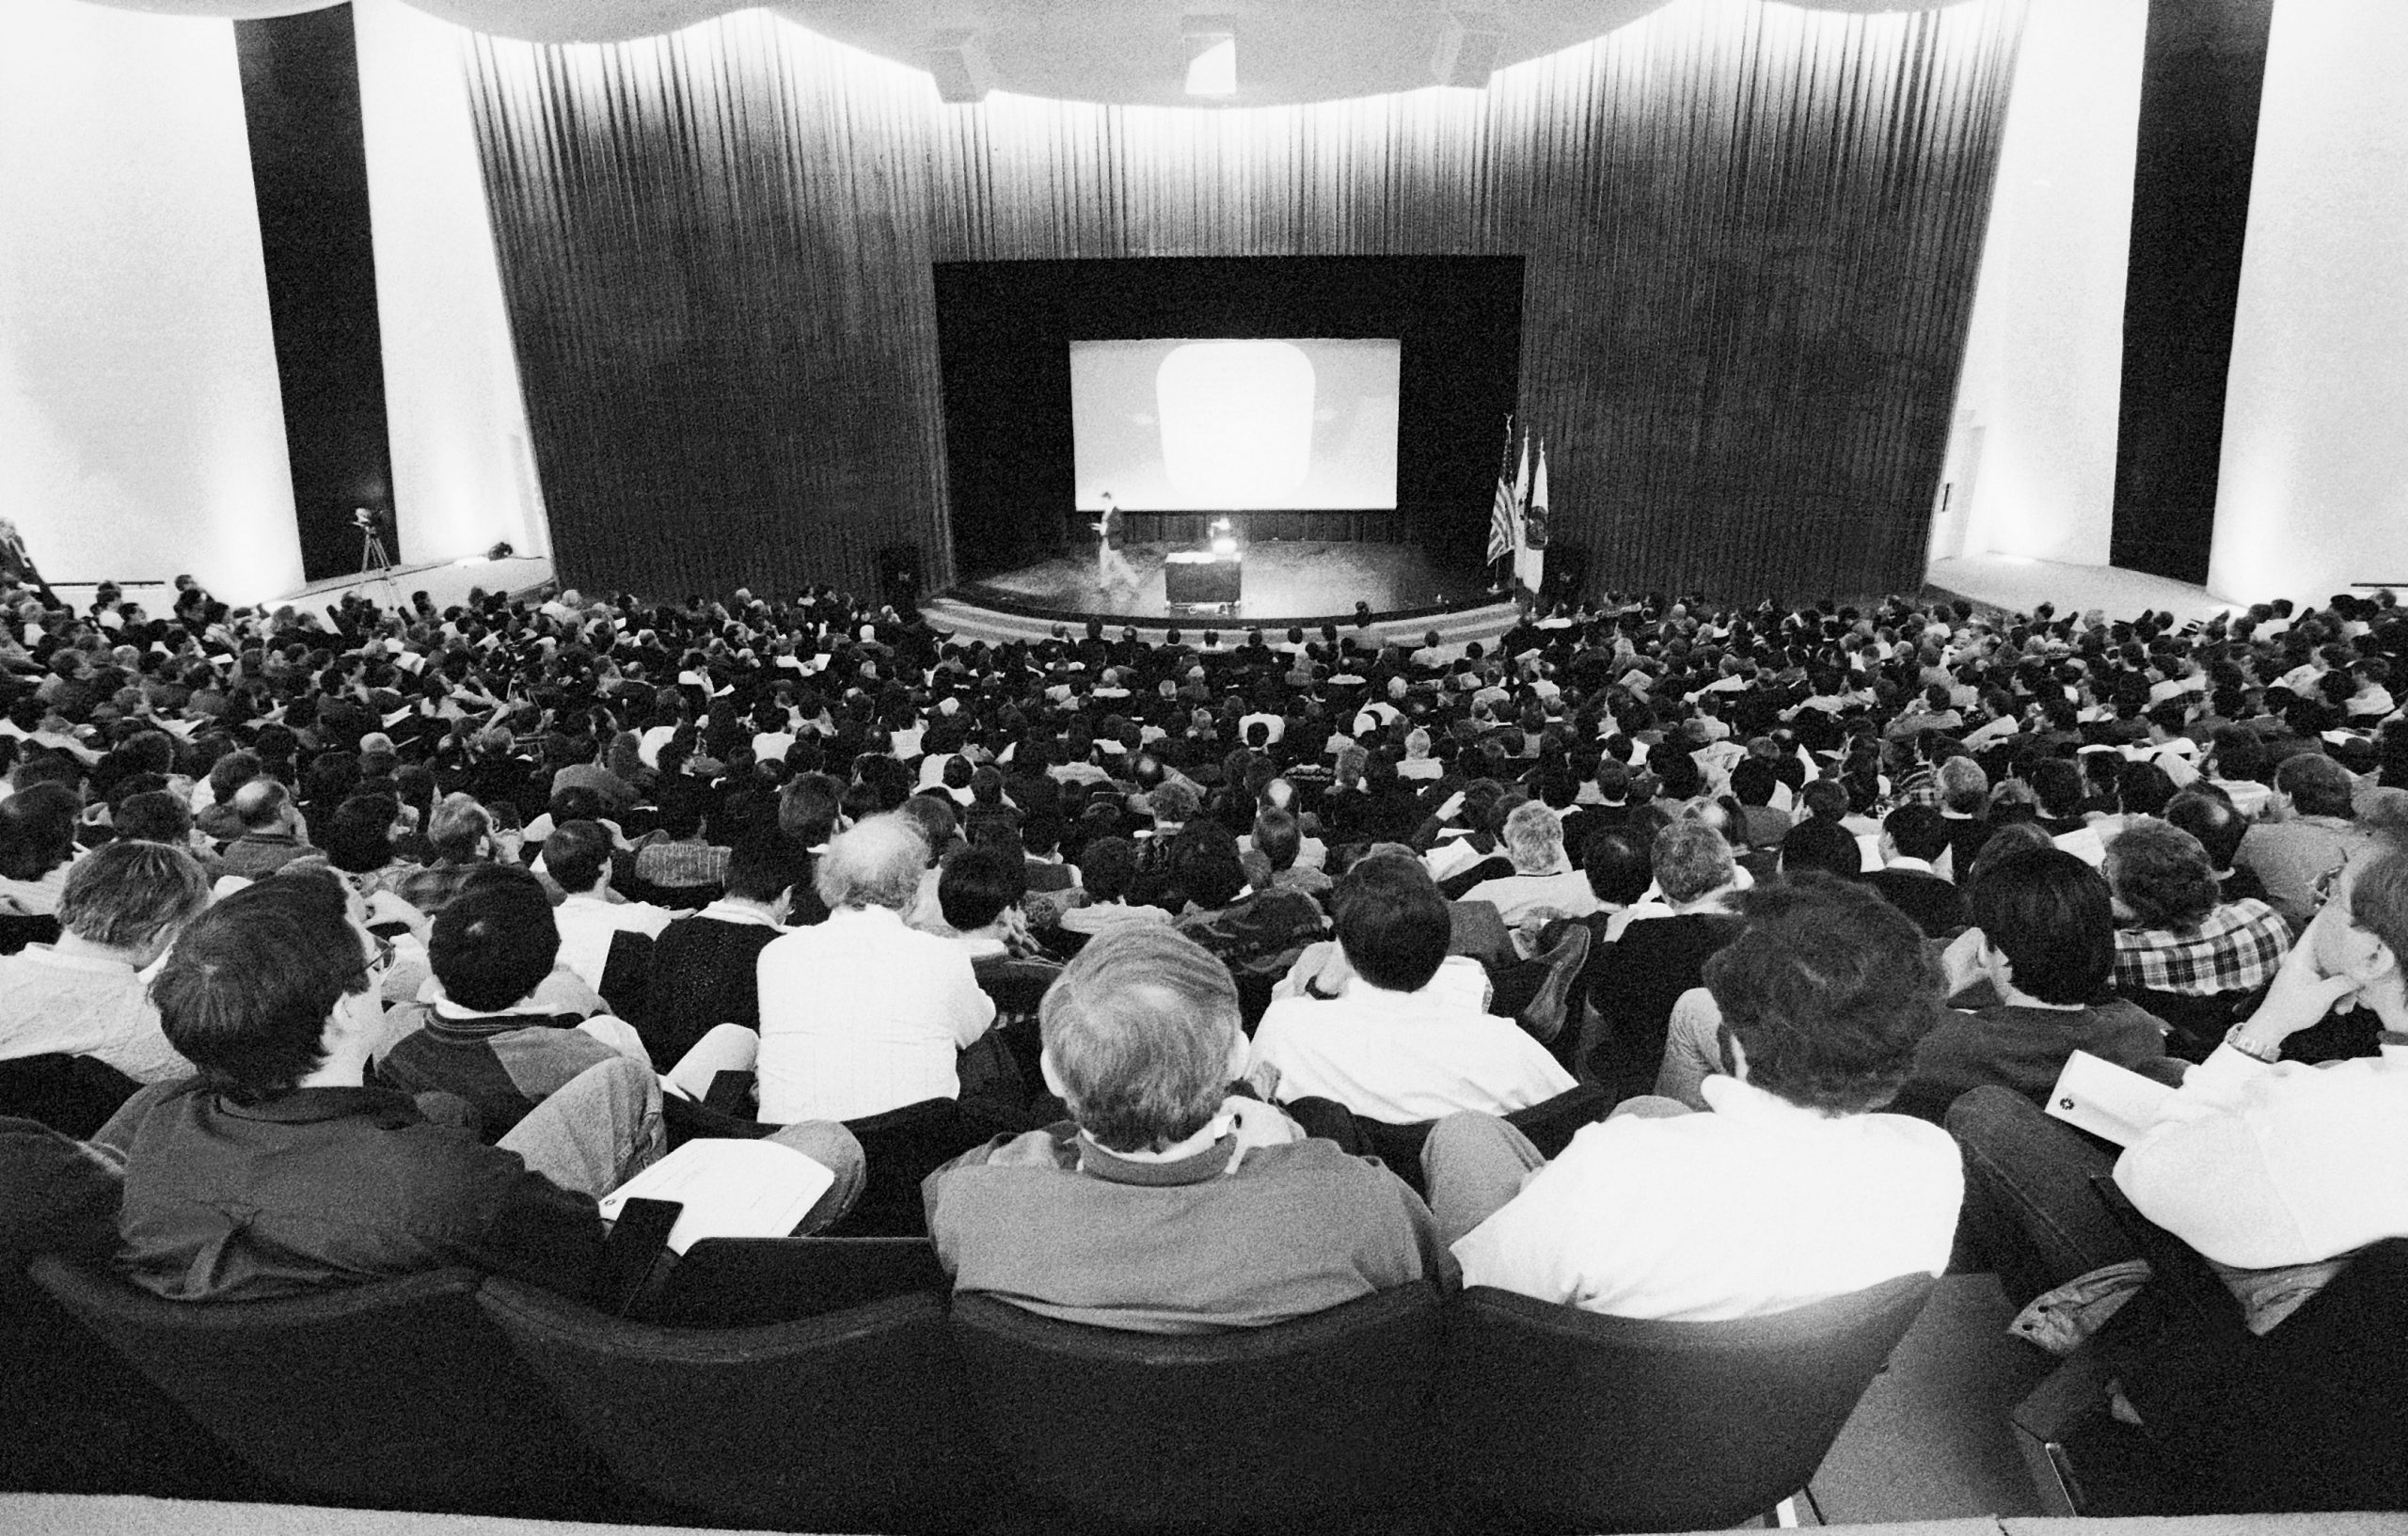
\includegraphics[width=0.5\textwidth]{./figures/TopQuark1.jpg}
        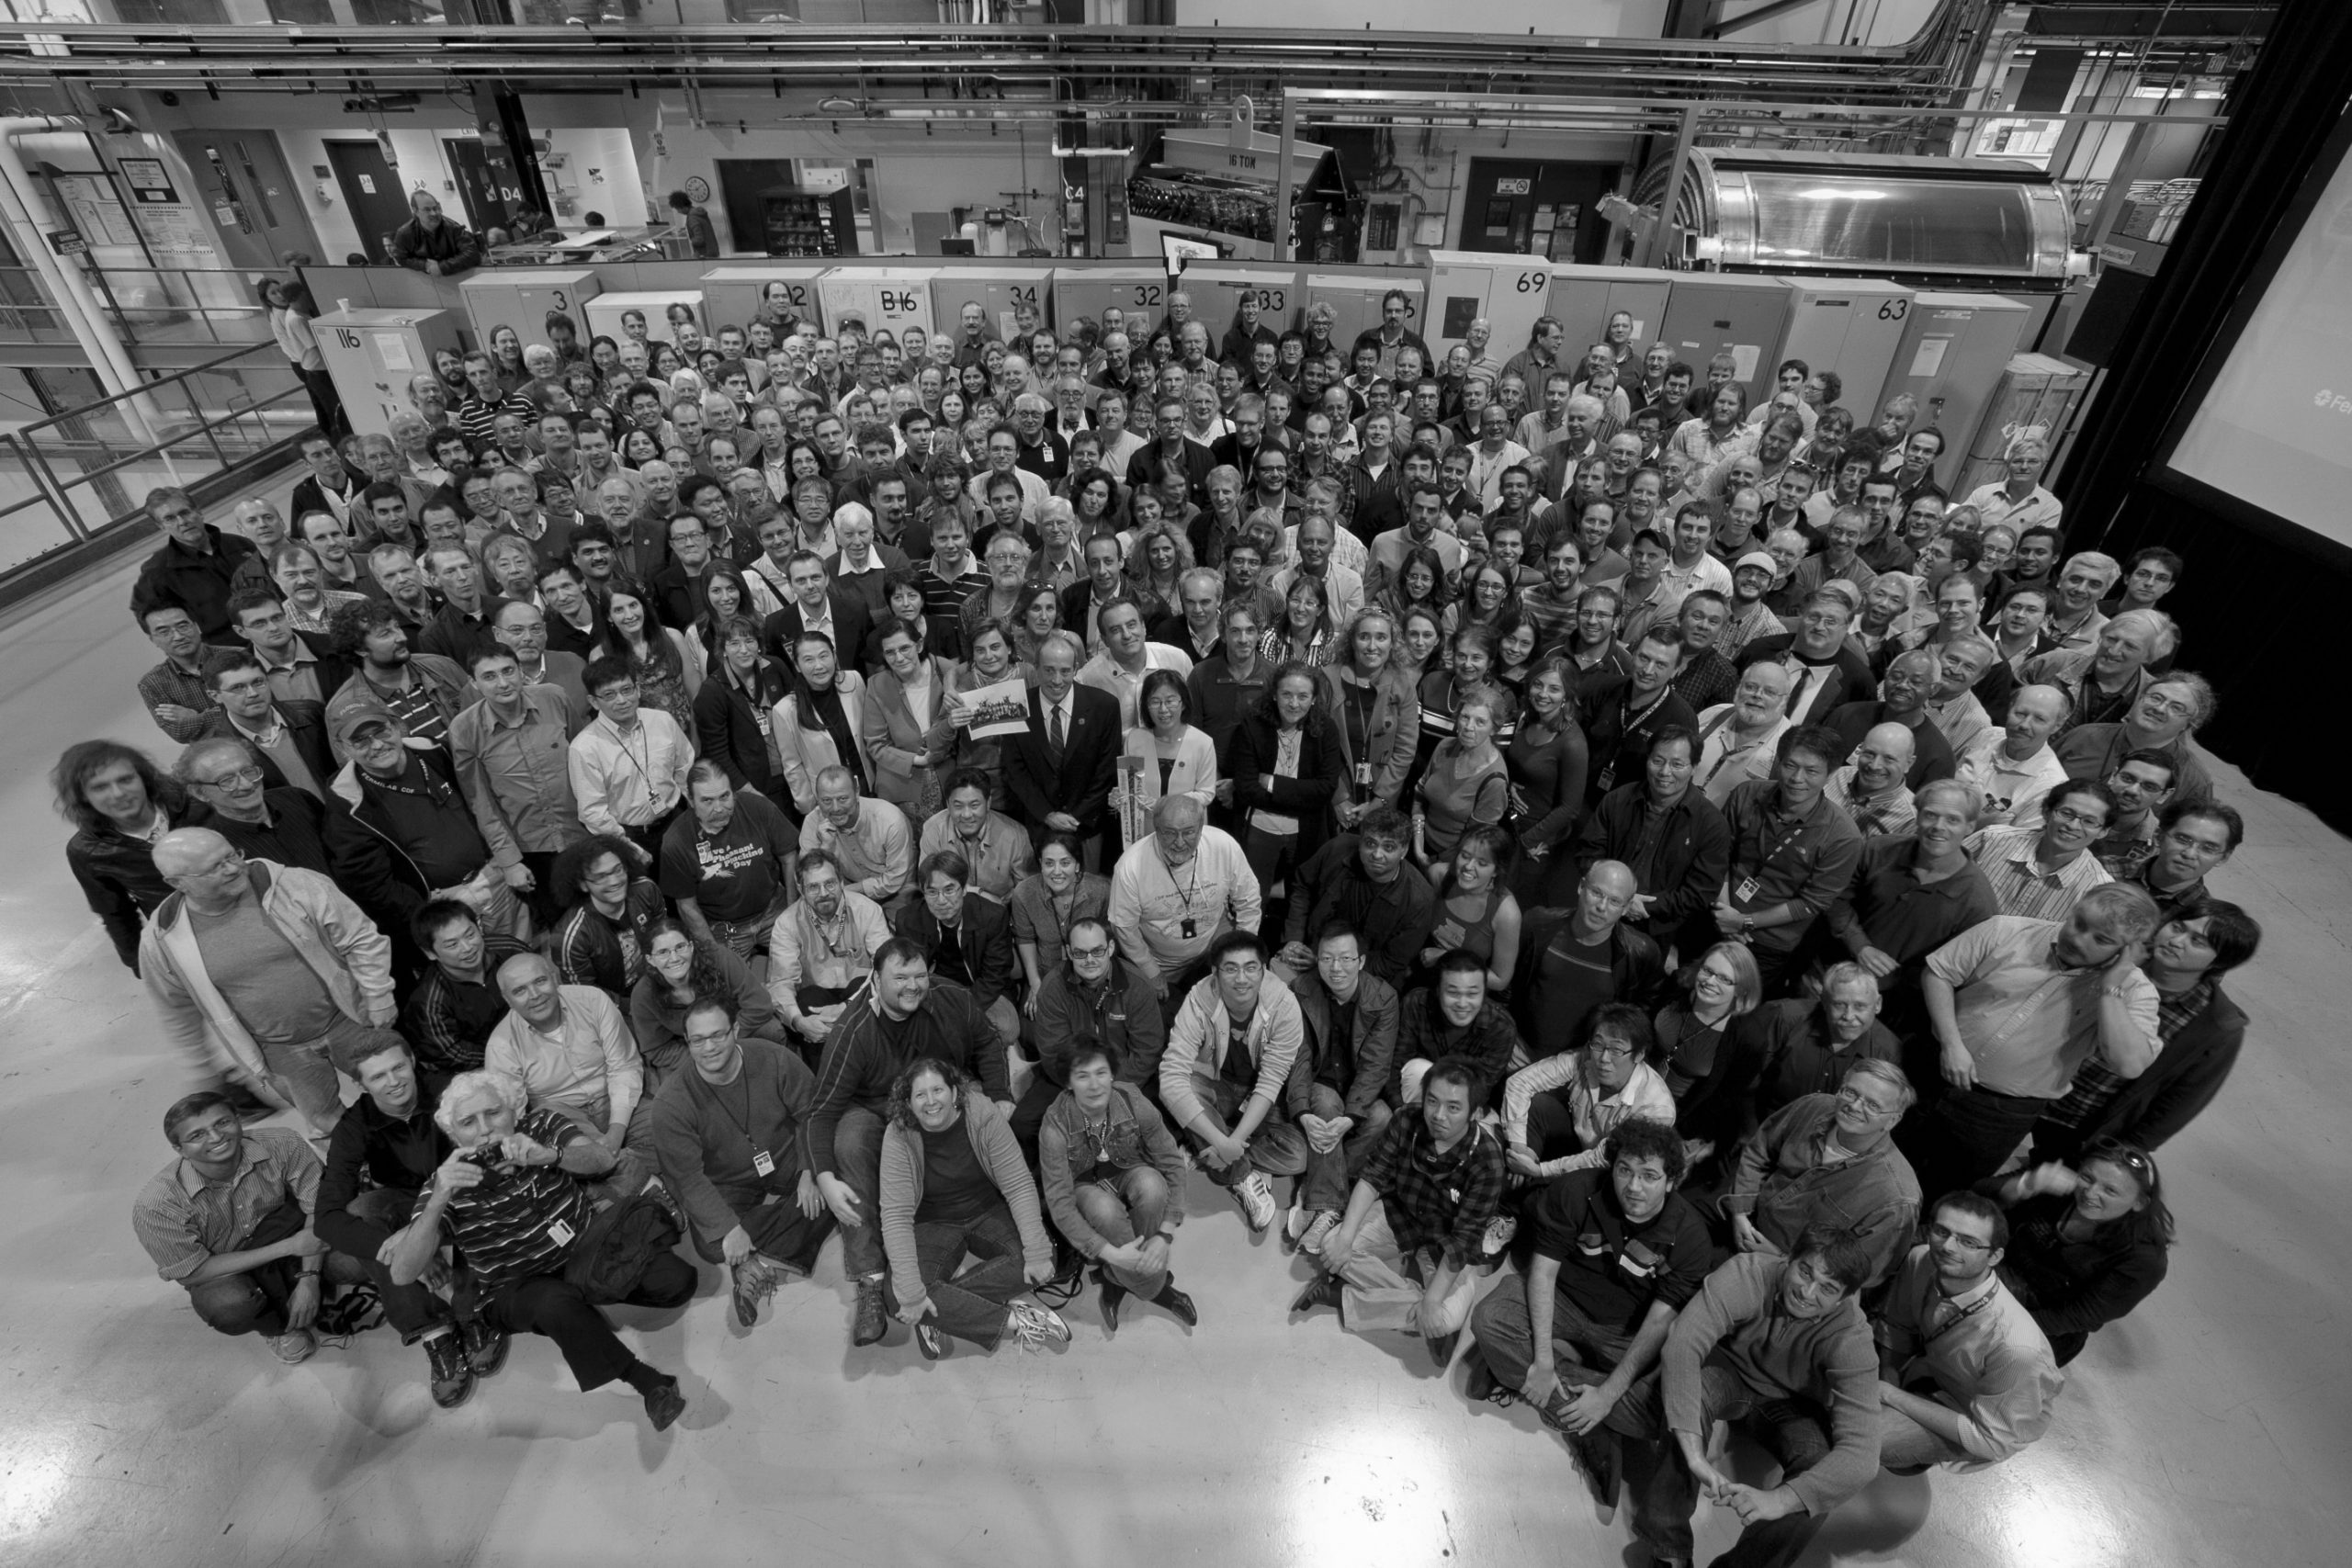
\includegraphics[width=0.5\textwidth]{./figures/TopQuark2BW.jpg}
      \end{center}
    \end{figure}
    % ========================
  \end{multicols}
\end{MyArticle}
